\documentclass{../../res/univ-projet}

\usepackage[utf8]{inputenc}
\usepackage[T1]{fontenc}
\usepackage[francais]{babel}

\logo{../../res/logo_univ.png}
\title{Plan de Développement}
\author{Adrien \bsc{Smondack}, Benjamin \bsc{Zigh}}
\projet{M1SSI}
\projdesc{Projet de génération d'OTP}
\filiere{M1SSI}
\version{3.0}
\relecteur{Gaëtan \bsc{Ferry}}
\signataire{Magali \bsc{Bardet}}
\date{Avril 2014}

\histentry{3.0}{07/04/2014}{Prise en compte des changements de fin d'itération.}
\histentry{2.0}{21/02/2014}{Version post état de l'art}
\histentry{1.3}{16/01/2014}{Version pour la revue de lancement.}
\histentry{1.2}{06/01/2014}{Version Finale.}
\histentry{1.1}{30/12/2013}{Version relue.}
\histentry{1.0}{19/12/2013}{Version initiale.}
\histentry{0.1}{06/12/2013}{Ébauche.}

\begin{document}
\maketitle

%----------------------------------------------------------------------------------------------------------------------------------------------
\section{Contexte du projet}
\subsection{Origine du projet}
	Ce projet a été mis en place en réponse à un appel d'offre concernant l'implémentation de système d'authentification via OTP par Magali \bsc{Bardet} et Bruno \bsc{Macadré}.
	
\subsection{Contexte du développement}
	\begin{description} 
		\item [Cadre :] Projet annuel de la formation M1SSI;
		\item [Période :] Novembre - Mai;
		\item [Contraintes :] Documents techniques et état de l'art rendus pour Janvier.
	\end{description}

\subsection{Acteurs}
	\begin{description}
		\item [Émetteur :] Mme \bsc{Bardet}, M. \bsc{Macadré};
		\item [Soutien technique :] Mme \bsc{Bardet}, Documentation.
		\item [Coach :] M. \bsc{Abdellah-Godard}
	\end{description}

\subsection{Objectifs poursuivis}
	\begin{itemize}
		\item Fournir un état de l'art sur les systèmes existants;
		\item Implémenter une ou plusieurs de ces méthodes;
		\item Garantir une sécurité forte.
	\end{itemize}

\subsection{Références}
	\begin{tabular}{p{1,5cm}>{\raggedright\arraybackslash}p{13cm}}
		{[ANS10]} & {ANSSI. Référentiel général de sécurité. \href{http://www.ssi.gouv.fr/fr/reglementation-ssi/referentiel-general-de-securite}{http://www.ssi.gouv.fr/fr/reglementation-ssi/referentiel-general-de-securite}, 2010.}
		\tabularnewline
		\\
		{[MvOV97]} & {Alfred J. Menezes, Paul C. van Oorschot, and Scott A. Vanstone. Handbook of applied cryptography. CRC Press Series on Discrete Mathematics and its Applications. CRC Press, Boca Raton, FL, 1997. With a foreword by Ronald L.Rivest.}
		\tabularnewline
		\\
		{[RFC98]} & {A One-Time Password System. \href{http://tools.ietf.org/html/rfc2289}{http://tools.ietf.org/html/rfc2289}, 1998.}
		\tabularnewline
		\\
		{[RFC05]} & {HOTP:An HMAC-Based One-Time Password Algorithm \href{http://tools.ietf.org/html/rfc4226}{http://tools.ietf.org/html/rfc4226}, 2005.}
		\tabularnewline
		\\
		{[RFC06]} & {Generic Message Exchange Authentication for the Securer Shell Protocol (SSH).\href{http://tools.ietf.org/html/rfc4256}{http://tools.ietf.org/html/rfc4256}, 2006.}
		\tabularnewline
		\\
		{[RFC07]} & {The EAP Protected One-Time Password Protocol (EAP-POTP). \href{http://tools.ietf.org/html/rfc4793}{http://tools.ietf.org/html/rfc4793}, 2007.}
		\tabularnewline
		\\
		{[RFC11]} & {TOTP: Time-Based One-Time Password Algorithm \href{http://tools.ietf.org/html/rfc6238}{http://tools.ietf.org/html/rfc6238}, 2011.}
		\tabularnewline
		\\
		{[goo]} & {Google Authenticator \href{https://code.google.com/p/google-authenticator/}{https://code.google.com/p/google-authenticator/}.}
	\end{tabular}
	
\newpage
%---------------------------------------------------------------------------------------------------------------------------------------------
\section{Méthodologie de développement}
\subsection{Le choix de la méthode}
	Nous avons comparé les différentes méthodes de développement vues en cours afin d'employer la mieux adaptée à notre projet. Parmi les méthodologies Agiles, qui nous étaient imposées, deux ont retenu notre attention: Scrum et eXtreme Programming (XP). En effet, ces deux méthodes sont bien adaptées à des équipes de taille réduite comme la notre. Nous avons donc comparé point par point les différents aspects de Scrum et XP.\\

	Comme mentionné précédemment, les deux ont l'avantage de bien s'adapter à des effectifs réduits comme le notre. XP est de plus pensé spécifiquement pour les projets de taille réduite. XP est plus orienté technique, avec des pratiques de codes établies tandis que Scrum met plus l'accent sur la gestion de projet pure et favorise la communication au sein de l'équipe.\\	

	Les différents comparatifs \footnote{\href{http://agile-only.com/master-thesis/software-dm/agile-s-dm/c-of-am}{http://agile-only.com/master-thesis/software-dm/agile-s-dm/c-of-am}}\footnote{\href{http://www.exa.unicen.edu.ar/catedras/agilem/comp.pdf}{http://www.exa.unicen.edu.ar/catedras/agilem/comp.pdf}} que nous avons pu étudier montrent que XP est généralement plus rapide mais plus couteux que Scrum. XP centre sa dynamique autour du client, tandis que Scrum favorise l'indépendance des équipes de développement.\\

	Au final, de nombreux critères nous ont orienté dans notre choix mais aucun n'a été plus important que la sécurité. Il s'agit en effet de l'objectif principal à atteindre pour un projet comme le notre et nous avons donc décidé de baser le choix de notre méthodologie dessus.\\
		
	Nous avons donc opté pour XP comme base, car cela semble le choix le plus cohérent pour un projet orienté sécurité, mais nous avons prévu d'adapter la méthode au contraintes de notre projet. En effet, les méthodes Agiles ne sont pas au point pour ce qui est des projets de sécurité informatique et les témoignages\footnote{\href{http://www.tripwire.com/state-of-security/security-data-protection/the-security-implications-of-agile-development/}{http://www.tripwire.com/state-of-security/security-data-protection/the-security-implications-of-agile-development/}} que nous avons pu recueillir préviennent que l'attachement à une méthode particulière peut se révéler contre-productif.\\

	Néanmoins, afin de nous prêter à l'évaluation du projet dans les meilleures conditions possibles, nous resterons au plus proche d'XP à travers tous le développement.
	
\subsection{eXtreme Programming: les grands principes}
	Il y a de nombreux principes qui composent l'eXtreme Programming, nous décrirons ici celles sur lesquelles nous comptons nous focaliser.

\subsubsection{Test Driven Development}
	Cette méthodologie liée à XP implique la création systématique de tests unitaires, automatisés si possible, pour chaque fonctionnalité. Le développement des composants vient après la création des tests et se déroule en gardant la satisfaction du test comme priorité en continu.\\

	Les développeurs doivent donc faire en sorte de satisfaire les exigences de qualité, tout en gardant leur code le plus simple possible, selon la philosophie K.I.S.S. \footnote{\href{http://en.wikipedia.org/wiki/KISS\_principle}{http://en.wikipedia.org/wiki/KISS\_principle}}.
	 
\subsubsection{Intégration Continue et Refactoring}
	Selon les principes d'intégration continue, on interface les composants entre eux au fur et à mesure du développement, afin de faciliter la livraison. Le refactoring  consiste à revoir régulièrement le code sans changer les fonctionnalités ou le comportement, ceci afin de produire du code facilement maintenable.

\subsubsection{Appropriation collective du code et programmation en binôme}
	Chaque membre de l'équipe devra être capable de travailler sur n'importe quelle partie du projet. La programmation se fera en binômes (deux par machine) afin de produire du code rigoureux et d'aider à faire progresser les membres plus faibles en technique.\\

	La revue de code sera effectuée régulièrement par les binômes sur le code des autres binômes, afin d'assurer le respect des conventions de codes fixées par le responsable technique et de faciliter l'intégration avec leur propre code.

\subsection{Étapes du développement}
	\begin{description}
		\item [Étape 1 :] État de l'art
			\begin{description}
		    	\item [Objectif :] Se familiariser avec les technologies actuelles et faire le point sur celles que l'on devra employer.
		        \item [Activité :] Étudier les RFC.
		        \item [Produit livrable :] Rapport.
		        \item [Responsabilité :] Toute l'équipe.
            \end{description}
	    \item [Étape 2 :] Algorithmes de calcul des OTP en C
		    \begin{description}
		        \item [Objectif :] Développer une bibliothèque capable de générer des OTP.
		        \item [Activité :] Suivre les algorithmes sélectionnés (conformément aux RFC).
		        \item [Produit livrable :] Bibliothèque C.
		        \item [Responsabilité :] La moitié de l'équipe.
		    \end{description}
	    \item [Étape 3 :] Algorithmes de calcul des OTP en Java
		    \begin{description}
		        \item [Objectif :] Développer une bibliothèque capable de générer des OTP.
		        \item [Activité :] Suivre les algorithmes sélectionnés (conformément aux RFC).
		        \item [Produit livrable :] Bibliothèque Java.
		        \item [Responsabilité :] La moitié de l'équipe.
		    \end{description}
	    \item [Étape 4 :] Implémentation de la gestion des utilisateurs en C
		    \begin{description}
		        \item [Objectif :] Pouvoir gérer des utilisateurs.
		        \item [Activité :] Créer la possibilité d'administrer les utilisateurs.
		        \item [Produit livrable :] Application de gestion utilisateur.
		        \item [Responsabilité :] La moitié de l'équipe.
		    \end{description}
	    \item [Étape 5 :] Implémentation de la gestion des Tokens en Java
		    \begin{description}
		        \item [Objectif :] Fournir un générateur d'OTP.
		        \item [Activité :] Intégration des outils et des modules de calculs d'OTP dans une IHM.
		        \item [Produit livrable :] Les tokens.
		        \item [Responsabilité :] La moitié de l'équipe.
		    \end{description}
	    \item [Étape 6 :] Implémentation des fonctions d'authentification de PAM
		    \begin{description}
		        \item [Objectif :] Permettre une connexion avec un OTP en vérifiant sa validité.
		        \item [Activité :] Mettre en place l'algorithme de comparaison de l'OTP reçut avec les données stockées.
		        \item [Produit livrable :] Le module d'authentification.
		        \item [Responsabilité :] La moitié de l'équipe.
	            \end{description}
	    \item [Étape 7 :] Création du GUI pour le Token android en Java
		    \begin{description}
		        \item [Objectif :] Fournir une interface au token.
		        \item [Activité :] Développer le GUI pour le Token.
		        \item [Produit livrable :] Les tokens.
		        \item [Responsabilité :] La moitié de l'équipe.
		    \end{description}
	    \item [Étape 8 :] Déploiement du Token sur SmartPhone
		    \begin{description}
		        \item [Objectif :] Token utilisable sur SmartPhone.
		        \item [Activité :] Intégrer le Token à un SmartPhone.
		        \item [Produit livrable :] Les tokens.
		        \item [Responsabilité :] La moitié de l'équipe.
		    \end{description}
	    \item [Étape 9 :] Création d'utilitaire en ligne de commande
		    \begin{description}
		        \item [Objectif :] Effectuer des opérations en ligne de commande.
		        \item [Activité :] Créer de nouvelles commandes.
		        \item [Produit livrable :] L'utilitaire.
		        \item [Responsabilité :] La moitié de l'équipe.
		    \end{description}
	    \item [Étape 10 :] Mise à jour du secret via PAM
		    \begin{description}
		        \item [Objectif :] Permettre la modification du secret.
		        \item [Activité :] Développement du module PAM permettant la modification du secret.
		        \item [Produit livrable :] Module PAM de mise à jour du secret.
		        \item [Responsabilité :] La moitié de l'équipe.
		    \end{description}
	    \item [Étape 11 :] Tests finaux, crash-test
		    \begin{description}
		        \item [Objectif :] Démontrer la force du système.
		        \item [Activité :] Tester l'application dans son ensemble et tenter des attaques sur le système.
		        \item [Produit livrable :] Le produit final.
		        \item [Responsabilité :] L'équipe.
		    \end{description}
    \end{description}
    
\newpage
%---------------------------------------------------------------------------------------------------------------------------------------------
\section{Organisation et responsabilités}
	\begin{figure}[h!]
		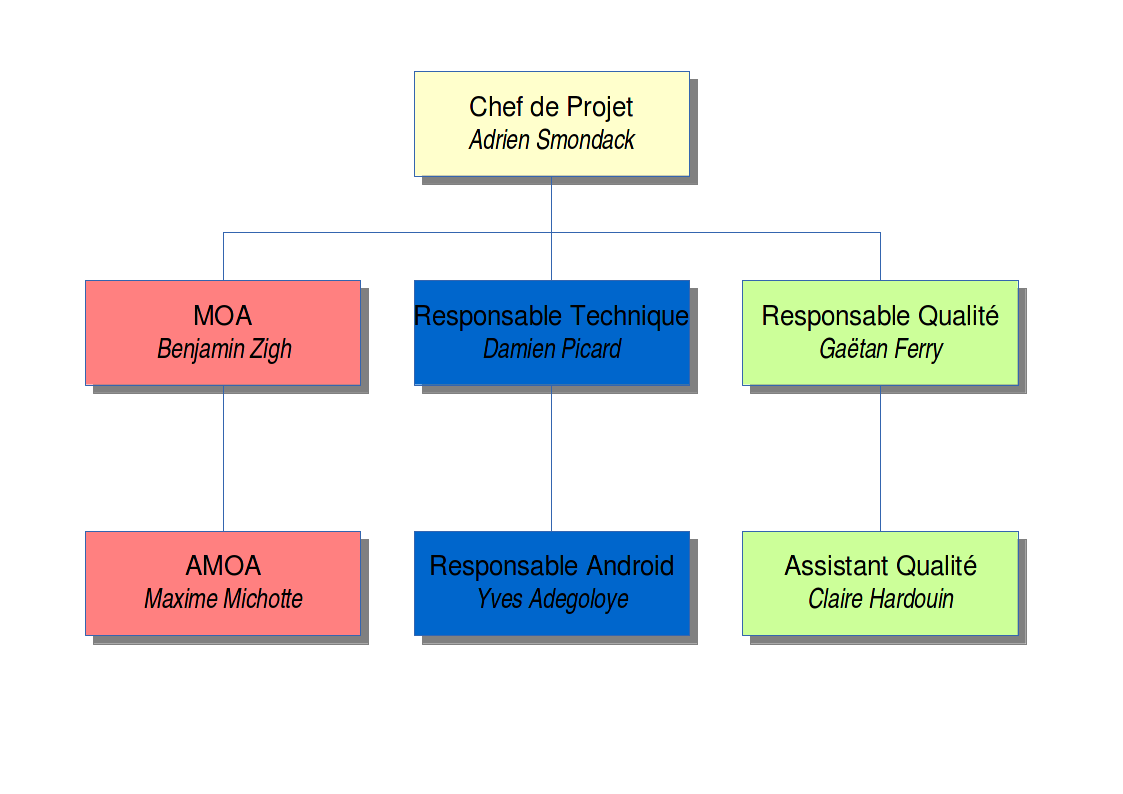
\includegraphics[scale=0.5]{organigramme.png}
		\caption{Organigramme des rôles au sein de l'équipe}
	\end{figure}
	
	\begin{description}
		\item[Chef de Projet :] Chargé de la coordination du projet et de la communication au sein de l'équipe.
		\item[Branche MOA :] Chargée de la communication entre l'équipe et le client.
		\item[Branche Technique :] Chargée de l'organisation du développement.
		\item[Branche Qualité :] Chargée du bon fonctionnement des livrables. 
	\end{description}
	
\newpage
%---------------------------------------------------------------------------------------------------------------------------------------------
\section{Organigramme des tâches}
	L'organisation suivante est déduite de l'état de l'art, qui n'est donc pas inclus.
	\begin{figure}[h]
		\begin{center}
			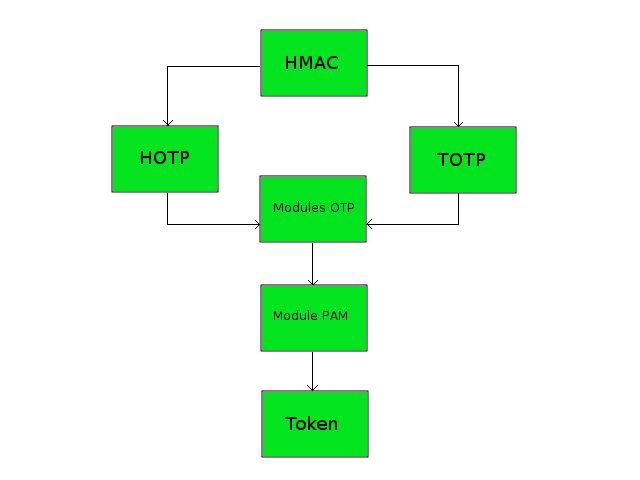
\includegraphics[scale=0.5]{taches.png}
			\caption{Organigramme des tâches à accomplir}
		\end{center}
	\end{figure}
	
	\begin{description}
		\item[HMAC :] Implémentations de HMAC pour différentes fonctions de hachage.
		\item[HOTP, TOTP :] Génération des OTP pour les protocoles choisis.
		\item[PAM :] Gestion centralisée des opérations d'authentifications.
		\item[Token :] Développement de l'interface utilisateur pour la génération d'OTP.
	\end{description}
	
\newpage
%---------------------------------------------------------------------------------------------------------------------------------------------
\section{Évaluation du projet et dimensionnement des moyens}
	Pour rappel, le projet peut être décomposé en 11 tâches distinctes :
	\begin{itemize}
	  \item Réalisation de l'état de l'art.
	  \item Implémentation des algorithmes de calcul des OTP en C.
	  \item Implémentation des algorithmes de calcul des OTP en JAVA.
	  \item Implémentation de la gestion des utilisateurs en C.
	  \item Implémentation de la gestion des Tokens en Java.
	  \item Implémentation des fonctions d'authentification de PAM.
	  \item Création du GUI pour le Token android en Java.
	  \item Déploiement du Token sur SmartPhone.
	  \item Création d'utilitaires en ligne de commande.
	  \item Mise à jour du secret via PAM.
	  \item Test finaux, crash-test.\\
	\end{itemize}

	Pour réaliser toutes ces tâches, on dispose de 169 jours complets de travail. Sur ces 169 jours, 7 collaborateurs travaillerons à temps plein sur le projet. Au total, nous disposons donc d'un total de 1183 jours-hommes de capacité de travail. Évaluons la charge requise pour chacune des taches :\\
	
	\begin{tabular}{|l|l|}
		\hline
		Tâche & Charges\\ 
		\hline
		État de l'art & 413 jours-hommes.\\
		Implémentation des algorithmes pour les calculs d'OTP en C & 96 jours-hommes.\\
		Implémentation des algorithmes pour les calculs d'OTP en JAVA & 72 jours-hommes.\\
		Implémentation de la gestion des utilisateurs en C & 80 jours-hommes.\\
		Implémentation des tokens en JAVA & 60 jours-hommes.\\
		Implémentation des fonctions d'authentification de PAM & 160 jours-hommes.\\
		Création d'une interface graphique pour le token Android & 60 jours-hommes.\\
		Déploiement des tokens Android sur smartphone & 15 jours-hommes.\\
		Création des utilitaires en ligne de commande & 39 jours-hommes.\\
		Mise à jour du secret via PAM & 91 jours-hommes.\\
		Tests finaux & 49 jours-hommes.\\ 
		\hline
	\end{tabular}
	
	\begin{tabular}{|l|l|l|}
	 	\hline
		Tâche & Durée & Ressources mobilisées \\ 
		\hline
		État de l'art & 59 Jours & 7 personnes \\
		Implémentation des algorithmes pour le calcul des OTP en C & 24 Jours & 4 personnes \\
		Implémentation des algorithmes pour le calcul des OTP en Java & 24 Jours & 3 personnes \\
		Implémentation de la gestion des utilisateurs en C. & 20 jours & 4 personnes \\
		Implémentation de la gestion des Tokens en Java. & 20 Jours & 3 personnes \\
		Implémentation des fonctions d'authentification de PAM. & 40 Jours & 4 personnes \\
	  	Création du GUI pour le Token android en Java. & 20 Jours & 3 personnes \\
		Déploiment du Token sur SmartPhone. & 5 Jours & 3 personnes \\
	  	Création d'utilitaire en ligne de commande. & 13 Jours & 3 personnes \\
	  	Mise à jour du secret via PAM. & 13 Jours & 7 personnes \\
		Tests finaux & 7 Jours & 7 personnes \\ 
		\hline
	\end{tabular}

\newpage
%---------------------------------------------------------------------------------------------------------------------------------------------
\section{Planning général}
	\begin{figure}[h!]
		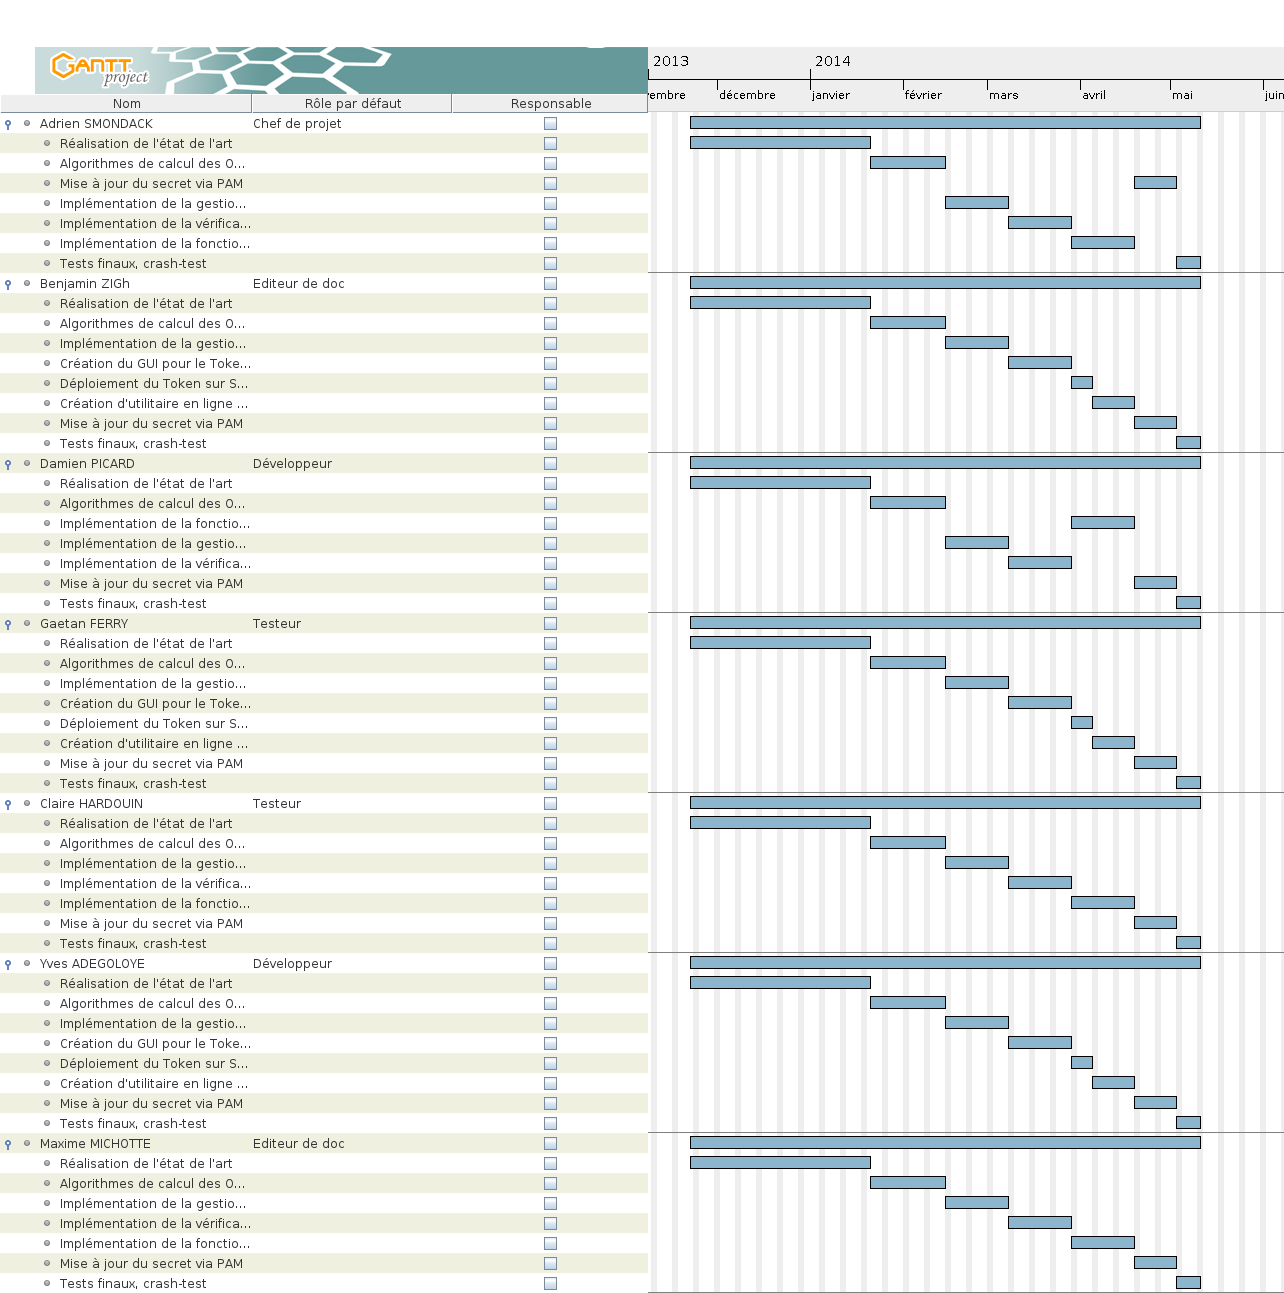
\includegraphics[scale=0.33]{ressources.png}
		\caption{Répartition des ressources sur le projet.}
	\end{figure}
	
	\newpage
	
	\begin{figure}[h!]
		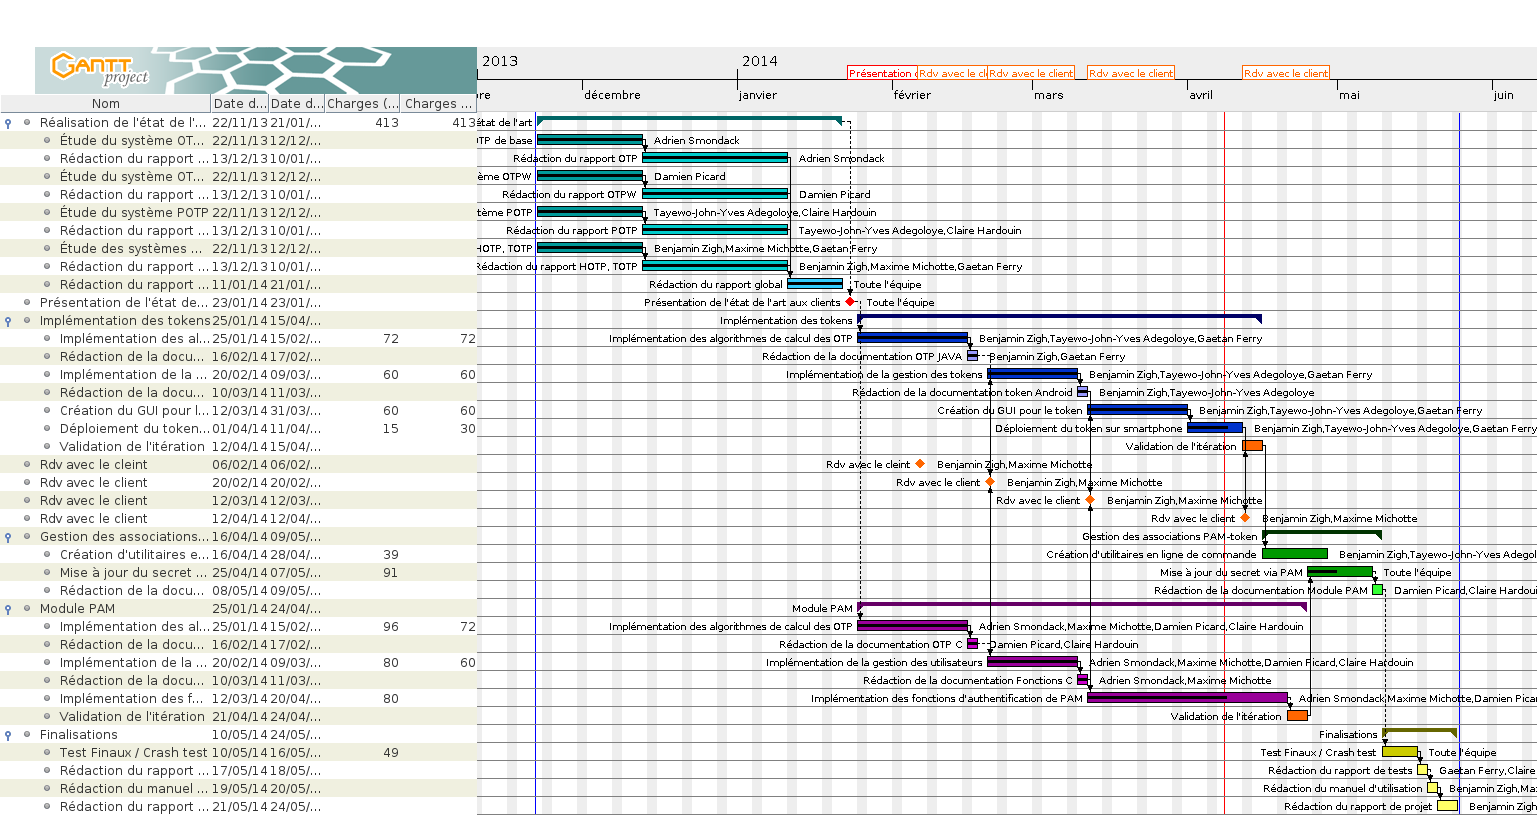
\includegraphics[scale=0.33]{gantt2-0.png}
		\caption{Planning des étapes du projet.}
	\end{figure}
	%\vspace{2cm}
	%\begin{figure}[h]
		%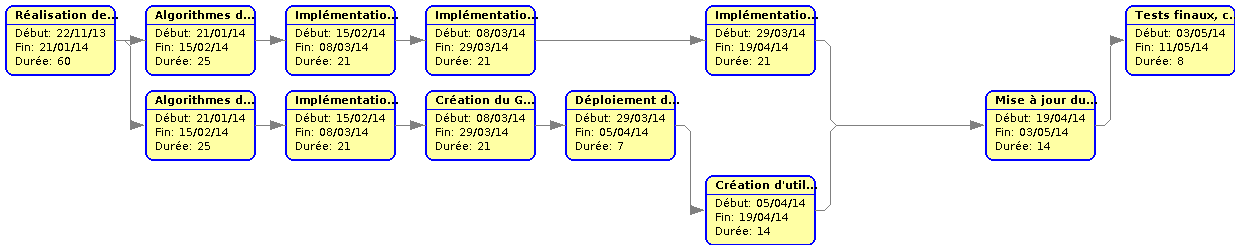
\includegraphics[scale=0.33]{pert.png}
		%\caption{Ordonnancement des tâches du projet.}
	%\end{figure}
	
	\newpage

%---------------------------------------------------------------------------------------------------------------------------------------------
\section{Procédés de gestion}
\subsection{Gestion de la documentation}
	\begin{tabular}{|l|l|l|}
		\hline
		Document & Rédaction & Relecture \\
		\hline
		Documentation OTP C & Damien \bsc{Picard} & Claire \bsc{Hardouin}\\
		Documentation OTP Java & Gaëtan \bsc{Ferry} & Benjamin \bsc{Zigh} \\
		Documentation Fonctions C & Adrien \bsc{Smondack} & Maxime \bsc{Michotte}\\
		Documentation Token Android & Yves \bsc{Adegoloye} & Benjamin \bsc{Zigh}\\
		Documentation Module PAM & Claire \bsc{Hardouin} & Damien \bsc{Picard} \\
		Rapports de tests & Gaëtan \bsc{Ferry} & Claire \bsc{Hardouin} \\
		Manuel d'utilisation & Benjamin \bsc{Zigh} & Maxime \bsc{Michotte} \\
		Rapport de projet & Maxime \bsc{Michotte} & Benjamin \bsc{Zigh} \\
		\hline 
	\end{tabular}

\subsection{Gestion des configurations}
\subsubsection{Gestion des versions}
	Nous avons choisi d'utiliser le logiciel git pour gérer les différentes versions du projet et des documents. À l'aide de celui-ci, nous pourrons aisément contrôler les étapes d'avancement du projet au cours de son développement. 

	Git permet de développer collaborativement à distance en enregistrant et/ou fusionnant les modifications apportées par les différents membres de l'équipe. Nous ne nous attarderons pas ici sur le fonctionnement de git (voir \href{http://git-scm.com/book/fr/Démarrage-rapide-Rudiments-de-Git}{http://git-scm.com/book/fr/Démarrage-rapide-Rudiments-de-Git}).

	La majorité de l'équipe était déjà formée à l'utilisation du logiciel, nous avons donc pu être opérationnels rapidement pour la rédaction des divers documents techniques.

	La gestion du git est attribuée au responsable technique.

\subsubsection{Hébergement}
	Github est un site d'hébergement de dépôts git proposant l'hébergement gratuit des projets publics. Il permet également aux étudiants de créer des projets privés dans un cadre universitaire.

	Le site est bien établi dans la communauté open-source et garantit une disponibilité de 99.9\%. Le fonctionnement de git nous permet en plus d'avoir chacun des versions locales, donc la perte de données ne représente pas un risque important.

	Encore une fois, la majorité des membres de l'équipe était déjà inscrite sur Github et il semblait logique de l'utiliser afin d'être efficace rapidement. 

	Github propose de nombreuses fonctionnalités supplémentaires, à la disposition du responsable technique pour communiquer avec l'équipe sur le développement du projet.

\newpage
%---------------------------------------------------------------------------------------------------------------------------------------------
\section{Revue et points clef}

\begin{description}
	\item Réalisation de l'état de l'art:
	\begin{description}
		\item[Objectifs :] Prendre connaissance des protocoles existants et de leur spécificités, puis déterminer ceux que nous utiliserons.
		\item[Prévisions :] Du 22/11/13 au 21/01/14.
		\item[Objet des vérifications :] Accord du client.
		\item[Modalité de contrôle :] Rapport détaillé sur chaque protocole étudié ainsi que nos conclusions.
		\item[Intervenants :] Toute l'équipe.
	\end{description}
	\vfill
	\item Algorithmes de calcul des OTP en C et Java:
	\begin{description}
		\item[Objectifs :] Concevoir des outils de calcul et de vérification d'OTP.
		\item[Prévisions :] Du 25/01/14 au 15/02/14 - État de l'art terminé.
<<<<<<< HEAD
		\item[Objet des vérifications :] Compilation du code + Tests.
=======
		\item[Objet des vérifications :] Compilation du code + tests.
>>>>>>> 6bead237b24919cc8bb70c8536ed5ca6c181229a
		\item[Modalité de contrôle :] Documentation à remettre au client.
		\item[Intervenants :] Par groupes.
	\end{description}
	\vfill
	\item Implémentation de la gestion des utilisateurs en C:
	\begin{description}
		\item[Objectifs :] Concevoir des outils de gestion des utilisateurs.
		\item[Prévisions :] Du 20/02/14 au 09/03/14 - Algorithmes de calcul disponibles.
		\item[Objet des vérifications :] Compilation du code + tests.
		\item[Modalité de contrôle :] Documentation à remettre au client.
		\item[Intervenants :] Par groupes.
	\end{description}
	\vfill
	\item Implémentation de la gestion des Tokens en Java:
	\begin{description}
		\item[Objectifs :] Fournir des générateurs d'OTP.
		\item[Prévisions :] Du 20/02/14 au 09/03/14 - Algorithmes de calcul disponibles.
		\item[Objet des vérifications :] Retour d'un OTP respectant les spécifications.
		\item[Modalité de contrôle :] Manuel d'utilisation et token à remettre au client.
		\item[Intervenants :] Par groupes.
	\end{description}
	\vfill
	\item Implémentation des fonctions d'authentification de PAM:
	\begin{description}
		\item[Objectifs :] Vérification de la validité d'un OTP reçut.
		\item[Prévisions :] Du 12/03/14 au 20/04/14 - Gestion utilisateurs + Tokens disponibles.
		\item[Objet des vérifications :] Compilation du code + tests.
		\item[Modalité de contrôle :] Module d'authentification à remettre au client.
		\item[Intervenants :] Par groupes.
	\end{description}
	\vfill
	\item Création du GUI pour le Token Android en Java:
	\begin{description}
		\item[Objectifs :] Fournir l'interface du token.
		\item[Prévisions :] Du 12/03/14 au 31/03/14 - Gestion utilisateurs + Tokens disponibles.
		\item[Objet des vérifications :] Compilation du code + tests.
		\item[Modalité de contrôle :] Manuel d'utilisation et token à remettre au client.
		\item[Intervenants :] Par groupes.
	\end{description}
	\vfill
	\item Déploiement du Token sur SmartPhone:
	\begin{description}
		\item[Objectifs :] Token utilisable sur SmartPhone.
		\item[Prévisions :] Du 01/04/14 au 06/04/14 - Vérification d'OTP disponible + Interface du token.
		\item[Objet des vérifications :] Tests.
		\item[Modalité de contrôle :] Token à remettre au client.
		\item[Intervenants :] Par groupes.
	\end{description}
	\vfill
	\item Implémentation de la fonction d'authentification sur PAM:
	\begin{description}
		\item[Objectifs :] Authentification à base d'OTP possible.
		\item[Prévisions :] Du 12/03/14 au 20/04/14 - Vérification d'OTP disponible + Interface du token.
		\item[Objet des vérifications :] Compilation du code + Tests.
		\item[Modalité de contrôle :] Module PAM d'authentification à remettre au client.
		\item[Intervenants :] Par groupes.
	\end{description}
	\vfill
	\item Création d'utilitaire en ligne de commande:
	\begin{description}
		\item[Objectifs :] Lignes de commandes opérationnelles.
		\item[Prévisions :] Du 16/04/14 au 28/04/14 - Vérification d'OTP disponible + Interface du token.
		\item[Objet des vérifications :] Tests.
		\item[Modalité de contrôle :] utilitaire à remettre au client.
		\item[Intervenants :] Par groupes.
	\end{description}
	\vfill
	\item Mise à jour du secret via PAM:
	\begin{description}
		\item[Objectifs :] Changement du secret possible.
		\item[Prévisions :] Du 25/04/14 au 07/05/14 - Authentification + utilitaire en ligne de commande disponible.
		\item[Objet des vérifications :] Compilation du code + Tests.
		\item[Modalité de contrôle :] Module PAM de mise à jour du secret à remettre au client.
		\item[Intervenants :] Par groupes.
	\end{description}
	\vfill
	\item Test finaux, crash-test:
	\begin{description}
		\item[Objectifs :] Assurer une sécurité mi-forte (authentification à deux facteurs).
		\item[Prévisions :] Du 10/05/14 au 16/05/14 - Authentifications possibles.
		\item[Objet des vérifications :] Résultat des tests positifs.
		\item[Modalité de contrôle :] Rapport de tests + Rapport de projet à remettre au client.
		\item[Intervenants :] Toute l'équipe.
	\end{description}
	\vfill
\end{description}

%---------------------------------------------------------------------------------------------------------------------------------------------
\section{Procédure de suivi et d'avancement}
	L'évolution du projet sera suivie en interne par : 
	\begin{itemize}
		\item des réunions régulières 
		\begin{description}
			\item[Objectif :] Faire le point sur l'avancement de chacun dans la tâche qui leur à été attribué et combler les lacunes qui pourraient se présenter.
			\item[Fréquence :] Toutes les deux semaines.
		\end{description}
		\item des séances de brainstorming par groupes
		\begin{description}
			\item[Objectif :] Décider des solutions à mettre en œuvre et de l'organisation du travail au sein du groupe pour résoudre la problématique.
			\item[Fréquence :] Aussi souvent que nécessaire.
		\end{description}
	\end{itemize}

	Côté client, l'avancement du projet pourra être suivi en permanence par l'intermédiaire du site d'hébergement Github. Ce procédé permettra aux clients de constater non seulement l'évolution de la documentation et des outils de développement, mais aussi d'avoir une idée plus précise sur la contribution de chaque groupe et de la régularité de leur travail.

	De plus, chaque étape débouchera sur la rédaction de documentation (compte-rendu ou manuel d'utilisation) dont une version imprimée sera remise en mains propres aux clients par la MOA.

	Outre les soutenances prévues en Janvier et en Mai, la MOA prévoit au minimum deux réunions par mois avec les clients pour faire le point sur l'avancement du projet et sur les besoins du client (pouvant entrainer une ré-actualisation de la documentation).

%---------------------------------------------------------------------------------------------------------------------------------------------
\end{document}
